\documentclass[12pt]{article}

\usepackage[margin=1in]{geometry}
\usepackage{amsmath,amsthm,amssymb,amsfonts,graphicx}
\usepackage{hyperref}
\usepackage{enumitem}

\newcommand{\Pp}{\emph{\emph{P}}}

\begin{document}

\title{Statistics Exam}
\author{Mr. Grant}
\maketitle

\begin{itemize}
	\item \textbf{Write your name}
	\item If you want partial credit for problems, show your work
	\item Good luck!
\end{itemize}

\begin{enumerate}[itemsep=-1ex]

	\item Mr. Grant is selecting a project team from the students Aaliyah, Akili, Brent, Branden, Booker, and Channing.
	\begin{itemize}
		\item If I randomly select just one person to join me for the project team, what is the probability that their name starts with an ``A?'' \vspace{10mm}
		\item I again randomly select one person for my team, but I've unfortunately become a sexist and won't work with girls (they have cooties). Given that I am not selecting a girl (assume that Channing and Aaliyah are the only girls in the group), what is the probability that the person selected's name starts with a ``B?'' \vspace{10mm}
		\item This time, I select two people for my group at random. What is the probability that I get Aaliyah and Akili (i.e. what is the probability that I get two people whose names both start with ``A'')? \vspace{15mm}
	\end{itemize}

	\item The mathematical constant $e = 2.71828182 \ldots$ is special for a variety of reasons (it is used by banks to calculate interest, for example). Consider each of the first 9 digits of $e$ as separate.
	\begin{itemize}
		\item What is the median of these digits? \vspace{10mm}
		\item The mean of the first 10 digits of $e$ is 4.7. What is the tenth digit of $e$? \vspace{10mm}
		%\item List the digits that are \textit{not} modes of the first 9 digits of $e$.
	\end{itemize}

	\newpage
\item The warp times, in milliseconds (as perceived from earth, so some times will actually be negative) for different spaceships' interdimensional travels are seen in this boxplot: 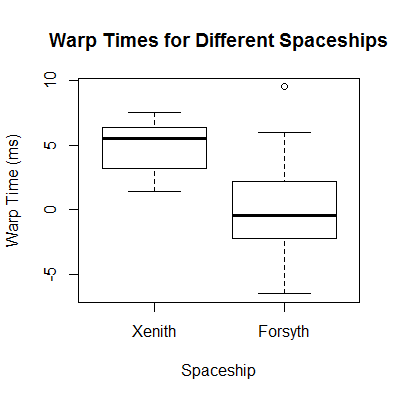
\includegraphics[scale=0.8]{boxplot} 
	\begin{itemize}
		% \item Which is larger: the first quartile of times for the Xenith, or the third quartile of times for the Forsyth?
		\item Fill in the blanks: the fastest \qquad percent of Forsyth warp times are faster than the slowest \qquad percent of Xenith warp times. There are many correct answers to this question; for full credit, give any of them, but for bonus, give an answer that conveys as much useful information as possible.
		\item Which spaceship's warp times are more variable? Why? \vspace{10mm}
	\end{itemize}

	\item This problem requires the use of R
	\begin{itemize}
		\item What is the average of the first 100 cubes (cubing a number is the same thing as raising it to the third power)? \vspace{5mm}
		\item The ``standard deviation'' of a vector of numbers is a way of measuring variability, and can be calculated in R using the \textit{sd()} function. To one decimal place (i.e. 2.7), what is the standard deviation of the first 9 digits of $e$ (treated as a vector)? 
	\end{itemize}

\item Josh and Pallas watched sidewalks in the U-district to see what kinds of people jaywalk. Name a kind of bias their study was \textbf{not} susceptible to, and explain why. \vspace{5mm}

\item Give a 1-sentence example of non-response bias. \vspace{10mm}

	\item A survey asks, ``Who is the better teacher, the illustrious genius Mr. Grant, or the lowly, dweeby Mr. Ben (who also has bad hair)?'' What kind of bias is in this survey question?

\end{enumerate}	

\end{document}
